\section{树}
\subsection{树的深度}
\lstinputlisting{图论/树/树的深度.cpp}

\subsection{二叉树还原}
\lstinputlisting{图论/树/二叉树还原.cpp}

\subsection{树的DFS序和欧拉序}
DFS序中一个点会出现一次,欧拉序会出现两次,两者都是 dfs 时经过的点的顺序,欧拉序中的第二次出现就是点结束搜索是回溯时的顺序
\lstinputlisting{图论/树/dfs序和欧拉序.cpp}

\subsection{树的重心}
对于\verb|size[i]|表示每个点子树大小,\verb|max_part(x)|表示删去\verb|x|后最大的子树的大小,\verb|max_part|取到最小值的点\verb|p|就是树的重心
\lstinputlisting{图论/树/树的重心.cpp}

\subsection{树上前缀和}
设\verb|sum[i]|表示节点\verb|i|到根节点的权值总和。

如果是点权,\verb|x,y|路径上的和为\verb|sum[x]+sum[y]-sum[lca]-sum[fa[lca]]|
\lstinputlisting{图论/树/树上前缀和_点.cpp}

如果是边权,\verb|x,y|路径上的和为\verb|sum[x]+sum[y]-2*sum[lca]|
\lstinputlisting{图论/树/树上前缀和_边.cpp}
\subsection{树上差分}
树上差分就是对树上某一段路径进行差分操作,树上差分分为\textbf{点差分}和\textbf{边差分}

这里的差分数组用\verb|d[i]|表示,其值是\verb|a[fa[i]]-a[i]|
\textbf{点差分}
\begin{center}
    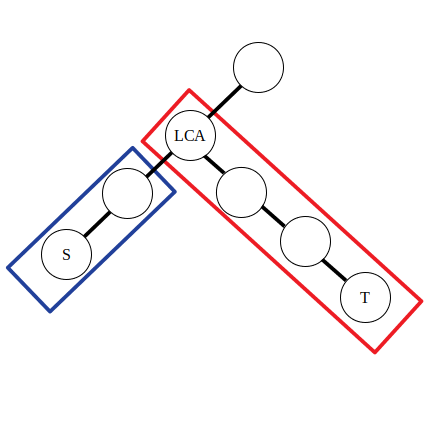
\includegraphics[scale=0.5]{图论/树/树上差分_点差分.png}
\end{center}

点差分实际上是要对链分成两条链来操作,如果要对\verb|(S,T)|路径上点权加\verb|p|

则要\verb|d[s] += p , d[t] += p , d[lca] -= p , d[ fa[lca] ] -= p|

\textbf{边差分}
\begin{center}
    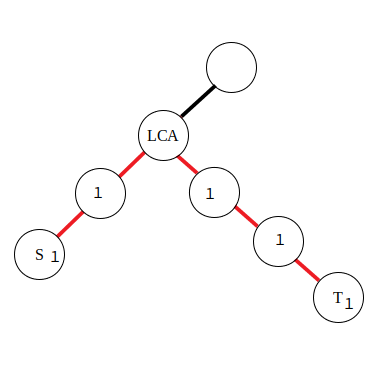
\includegraphics[scale=0.5]{图论/树/树上差分_边差分}
\end{center}

因为直接对边差分比较困难,所以要把边权移动到边上的子节点上,如果要对\verb|(S,T)|路径上边权加\verb|p|,则要\verb|d[s] += p , d[t] += p , d[lca] -= 2 * p|

\lstinputlisting{图论/树/树上差分_边差分.cpp}